% Options for packages loaded elsewhere
\PassOptionsToPackage{unicode}{hyperref}
\PassOptionsToPackage{hyphens}{url}
%
\documentclass[
]{article}
\usepackage{amsmath,amssymb}
\usepackage{lmodern}
\usepackage{float}
\usepackage{iftex}
\ifPDFTeX
  \usepackage[T1]{fontenc}
  \usepackage[utf8]{inputenc}
  \usepackage{textcomp} % provide euro and other symbols
\else % if luatex or xetex
  \usepackage{unicode-math}
  \defaultfontfeatures{Scale=MatchLowercase}
  \defaultfontfeatures[\rmfamily]{Ligatures=TeX,Scale=1}
\fi
% Use upquote if available, for straight quotes in verbatim environments
\IfFileExists{upquote.sty}{\usepackage{upquote}}{}
\IfFileExists{microtype.sty}{% use microtype if available
  \usepackage[]{microtype}
  \UseMicrotypeSet[protrusion]{basicmath} % disable protrusion for tt fonts
}{}
\makeatletter
\@ifundefined{KOMAClassName}{% if non-KOMA class
  \IfFileExists{parskip.sty}{%
    \usepackage{parskip}
  }{% else
    \setlength{\parindent}{0pt}
    \setlength{\parskip}{6pt plus 2pt minus 1pt}}
}{% if KOMA class
  \KOMAoptions{parskip=half}}
\makeatother
\usepackage{xcolor}
\usepackage[margin=1in]{geometry}
\usepackage{graphicx}
\makeatletter
\def\maxwidth{\ifdim\Gin@nat@width>\linewidth\linewidth\else\Gin@nat@width\fi}
\def\maxheight{\ifdim\Gin@nat@height>\textheight\textheight\else\Gin@nat@height\fi}
\makeatother
% Scale images if necessary, so that they will not overflow the page
% margins by default, and it is still possible to overwrite the defaults
% using explicit options in \includegraphics[width, height, ...]{}
\setkeys{Gin}{width=\maxwidth,height=\maxheight,keepaspectratio}
% Set default figure placement to htbp
\makeatletter
\def\fps@figure{htbp}
\makeatother
\setlength{\emergencystretch}{3em} % prevent overfull lines
\providecommand{\tightlist}{%
  \setlength{\itemsep}{0pt}\setlength{\parskip}{0pt}}
\setcounter{secnumdepth}{-\maxdimen} % remove section numbering
\ifLuaTeX
  \usepackage{selnolig}  % disable illegal ligatures
\fi
\IfFileExists{bookmark.sty}{\usepackage{bookmark}}{\usepackage{hyperref}}
\IfFileExists{xurl.sty}{\usepackage{xurl}}{} % add URL line breaks if available
\urlstyle{same} % disable monospaced font for URLs
\hypersetup{
  pdftitle={ecpn\_appendix},
  hidelinks,
  pdfcreator={LaTeX via pandoc}}

\title{ecpn\_appendix}
\author{}
\date{\vspace{-2.5em}}

\begin{document}
\maketitle

\hypertarget{appendix-a-randomization-inference-and-bootstrapping}{%
\subsection{Appendix A: Randomization Inference and
Bootstrapping}\label{appendix-a-randomization-inference-and-bootstrapping}}

Randomization inference and bootstrapping are nonparametric methods to
generate \(p\)-values (randomization inference) and confidence intervals
(bootstrapping). With \emph{randomization inference}, we first shuffle
the treatment variable to break the relationship between treatment and
outcomes. Next we regress outcomes on treatment using our regression
equation and store the resulting coefficient. Lastly, we repeat that
process 10,000 times to create the distribution of coefficients we would
observe if treatment had no effect on outcomes -- the null hypothesis.
Our \(p\)-value is the proportion of the null distribution that is
greater than or equal to our observed coefficient.

\emph{Bootstrapping} for standard errors is similar, but instead of
shuffling the treatment indicator we resample units with replacement. By
resampling with replacement, we create the empirical distribution of our
data and the range of possible treatment effects we might observe if we
repeated the experiment 10,000 times. The treatment effect at the 2.5th
percentile and at the 97.5th percentile are equivalent to a 95\%
confidence interval {[}@efron1994introduction{]}.

In each of these procedures, we mimic our randomization process by
randomizing/resampling the intervention to communities in site-level
clusters and within state blocks. This means that both communities in an
implementation site (farmers and pastoralists) will always be
treated/sampled together and that assignment to the intervention and
resampling are conducted separately in Nassarawa and Benue, just as the
intervention was assigned in this study. This procedure ensures that our
null distribution (for \(p\)-values) is created by randomizing the
intervention between exchangeable units and that our empirical
distribution (for confidence intervals) is created by resampling units
as they were sampled.

\begin{center}\rule{0.5\linewidth}{0.5pt}\end{center}

\hypertarget{appendix-b-robustness-checks-for-community-analysis}{%
\subsection{Appendix B: Robustness checks for community
analysis}\label{appendix-b-robustness-checks-for-community-analysis}}

These tables shows results with different ways of making indices
(additive vs inverse-covariance weighted), different models for
estimating effects (differencing vs controlling-for), and different ways
of coding count variables (raw vs ranked). Each table is an outcome.
Rows are results for different ways of creating the outcomes. Columns
show the coefficient from OLS regression, true p-value from
randomization inference, and a binary ``base'' indicator showing which
method was used in the paper.

The base method is always inverse-covariance weighted indices; the
estimation method is controlling-for unless the baseline difference
between the treatment and control groups is 0.20 standard deviations or
more; the base method of handling count variables is dense rank. Only
contact outcomes use count variables, only survey outcomes have a
baseline and an endline and are measured with indices.

\begin{table}[H]
\begin{center}
\label{tab:attitude_tab}
\caption{\textbf{Community Attitudes.} Effect of ECPN on attitudes using alternative methods of estimation and index construction. The first column shows coefficients from OLS regression, the second column shows $p$-values from randomization inference, and the third column shows which method was used in the paper.}
\smallskip

\begin{tabular}{l|r|r|r}
\hline
  & coefficient & p-value & base\\
\hline
Controlling-for \& ICW & 0.116 & 0.045 & 1\\
\hline
Controlling-for \& Additive & 0.093 & 0.038 & 0\\
\hline
Differencing \& ICW & 0.100 & 0.145 & 0\\
\hline
Differencing \& Additive & 0.073 & 0.116 & 0\\
\hline
\end{tabular}


\end{center}
\end{table}

\begin{table}[H]
\begin{center}
\label{tab:security_tab}
\caption{\textbf{Community Perceptions of Security} Effect of ECPN on perceptions of security using alternative methods of estimation and index construction. The first column shows coefficients from OLS regression, the second column shows $p$-values from randomization inference, and the third column shows which method was used in the paper.}
\smallskip

\begin{tabular}{l|r|r|r}
\hline
  & coefficient & p-value & base\\
\hline
Controlling-for \& ICW & 0.098 & 0.032 & 0\\
\hline
Controlling-for \& Additive & -0.010 & 0.593 & 0\\
\hline
Differencing \& ICW & 0.159 & 0.020 & 1\\
\hline
Differencing \& Additive & 0.054 & 0.213 & 0\\
\hline
\end{tabular}


\end{center}
\end{table}

\begin{table}[H]
\begin{center}
\label{tab:contact_tab}
\caption{\textbf{Community Contact} Effect of ECPN on contact using alternative methods of estimation, index construction, and measuring count variables. The first column shows coefficients from OLS regression, the second column shows $p$-values from randomization inference, and the third column shows which method was used in the paper.}
\smallskip

\begin{tabular}{l|r|r|r}
\hline
  & coefficient & p-value & base\\
\hline
Controlling-for \& ICW \& Ranks & 0.013 & 0.424 & 0\\
\hline
Controlling-for \& Additive \& Ranks & 0.003 & 0.422 & 0\\
\hline
Differencing \& ICW \& Ranks & 0.138 & 0.060 & 1\\
\hline
Differencing \& Additive \& Ranks & 0.015 & 0.182 & 0\\
\hline
Controlling-for \& ICW \& Categories & 0.017 & 0.377 & 0\\
\hline
Controlling-for \& ICW \& Raw & -0.020 & 0.602 & 0\\
\hline
Differencing \& ICW \& Categories & 0.120 & 0.064 & 0\\
\hline
Differencing \& ICW \& Raw & 0.071 & 0.207 & 0\\
\hline
\end{tabular}


\end{center}
\end{table}

\begin{table}[H]
\begin{center}
\label{tab:percExp_tab}
\caption{\textbf{Community Contact Willingness (Percent Experiment)} Effect of ECPN on willingness to have contact with the outgroup using alternative methods of estimation. The first column shows coefficients from OLS regression, the second column shows $p$-values from randomization inference, and the third column shows which method was used in the paper.}
\smallskip

\begin{tabular}{l|r|r|r}
\hline
  & coefficient & p-value & base\\
\hline
Controlling-for & 0.093 & 0.051 & 0\\
\hline
Differencing & 0.062 & 0.239 & 1\\
\hline
\end{tabular}


\end{center}
\end{table}

\begin{figure}[H]
\begin{center}
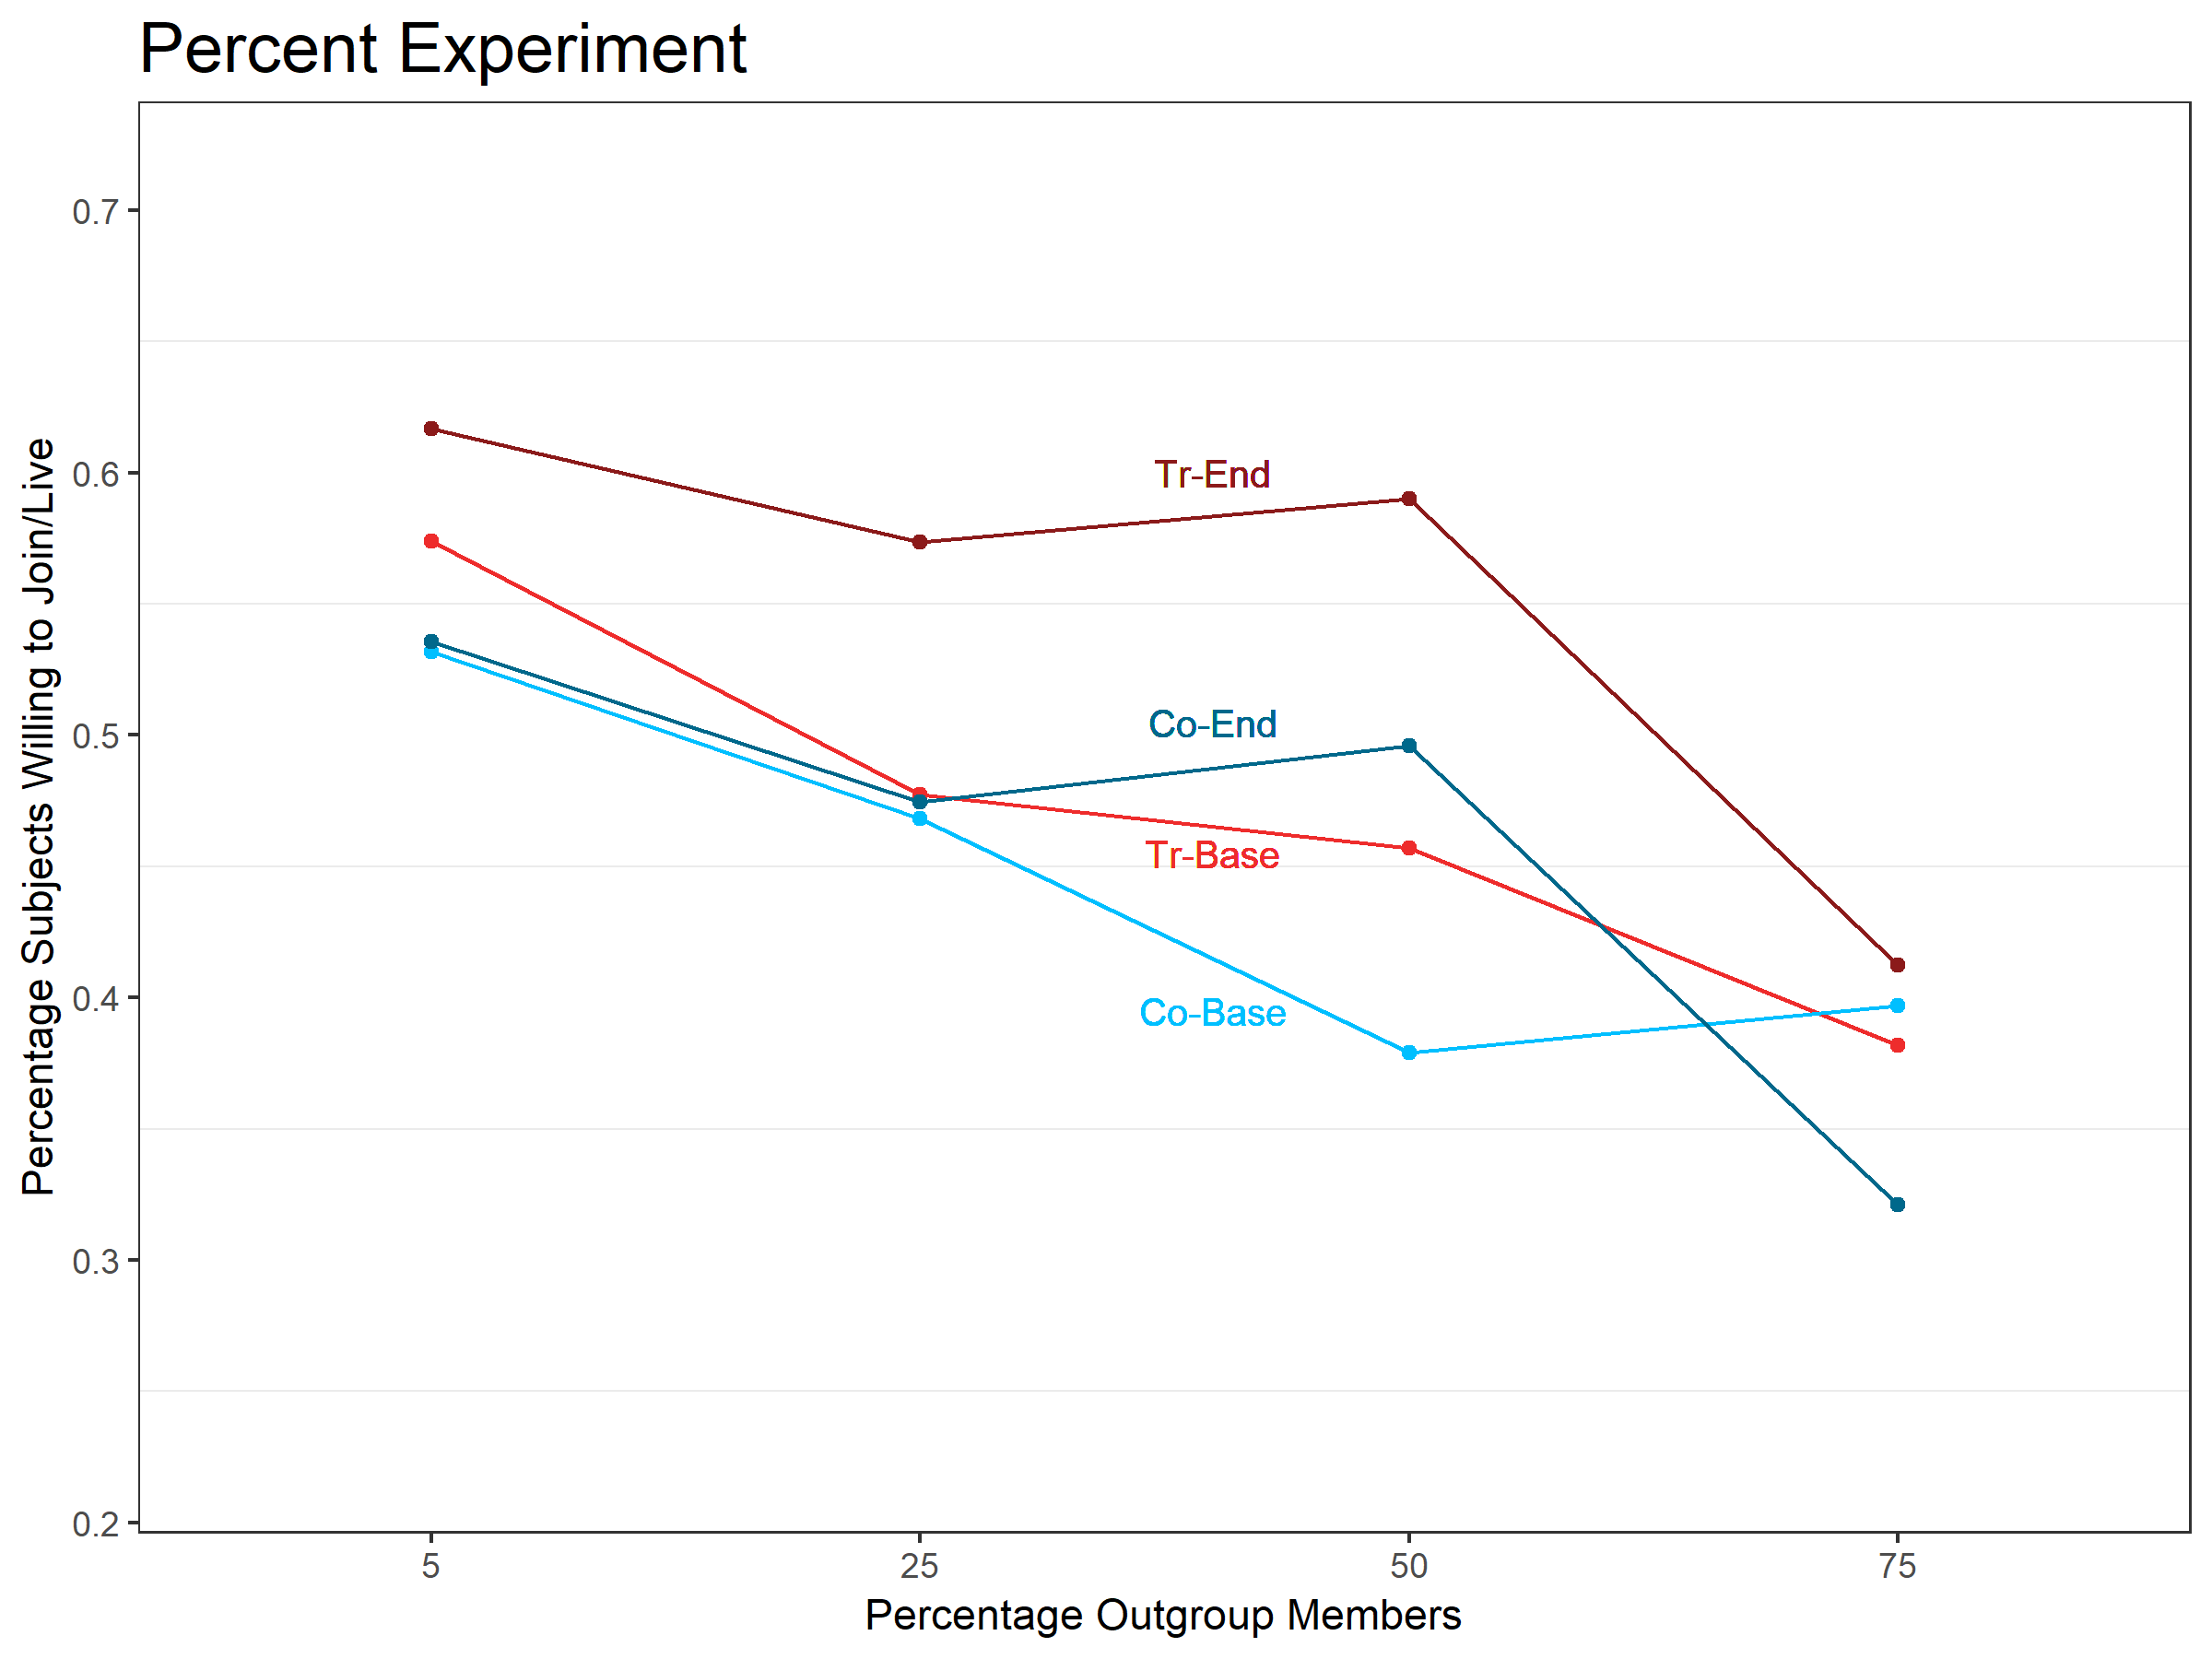
\includegraphics[width=.8\textwidth]{figs/randComm_plot.png}
\caption{\label{fig:percExp_plot_comm} \textbf{Community Percent Experiment} This figure shows the proportion of each experimental group who would join a group or live in a community with increasing percentages of outgroup members. The outcome is the mean response of those two questions so that a respondent saying yes to both was assigned a 1, a respondent saying yes to one was assigned a 0.5, and a respondent saying no to both was assigned a 0. Red shows the treatment communities; blue shows control communities.  Light colors are values at baseline; dark colors are values at endline.}
\end{center}
\end{figure}

\begin{table}[H]
\begin{center}
\label{tab:endExp_tab}
\caption{\textbf{Community Endorsement Experiment} Effect of ECPN on endorsement experiment using alternative methods of estimation. The first column shows coefficients from OLS regression, the second column shows $p$-values from randomization inference, and the third column shows which method was used in the paper.}
\smallskip

\begin{tabular}{l|r|r|r}
\hline
  & coefficient & p-value & base\\
\hline
Controlling-for & 0.103 & 0.158 & 0\\
\hline
Differencing & 0.123 & 0.212 & 1\\
\hline
\end{tabular}


\end{center}
\end{table}

\begin{table}[H]
\begin{center}
\label{tab:pgg_tab}
\caption{\textbf{Community Public Goods Game} Effect of ECPN on probability of donating and on donation amount. The first column shows coefficients from OLS regression and the second column shows $p$-values from randomization inference.}
\smallskip

\begin{tabular}{l|r|r}
\hline
  & coefficient & p-value\\
\hline
Donation (binary) & 0.022 & 0.294\\
\hline
Donation amount & -35.124 & 0.852\\
\hline
\end{tabular}


\end{center}
\end{table}

\begin{figure}[H]
\begin{center}
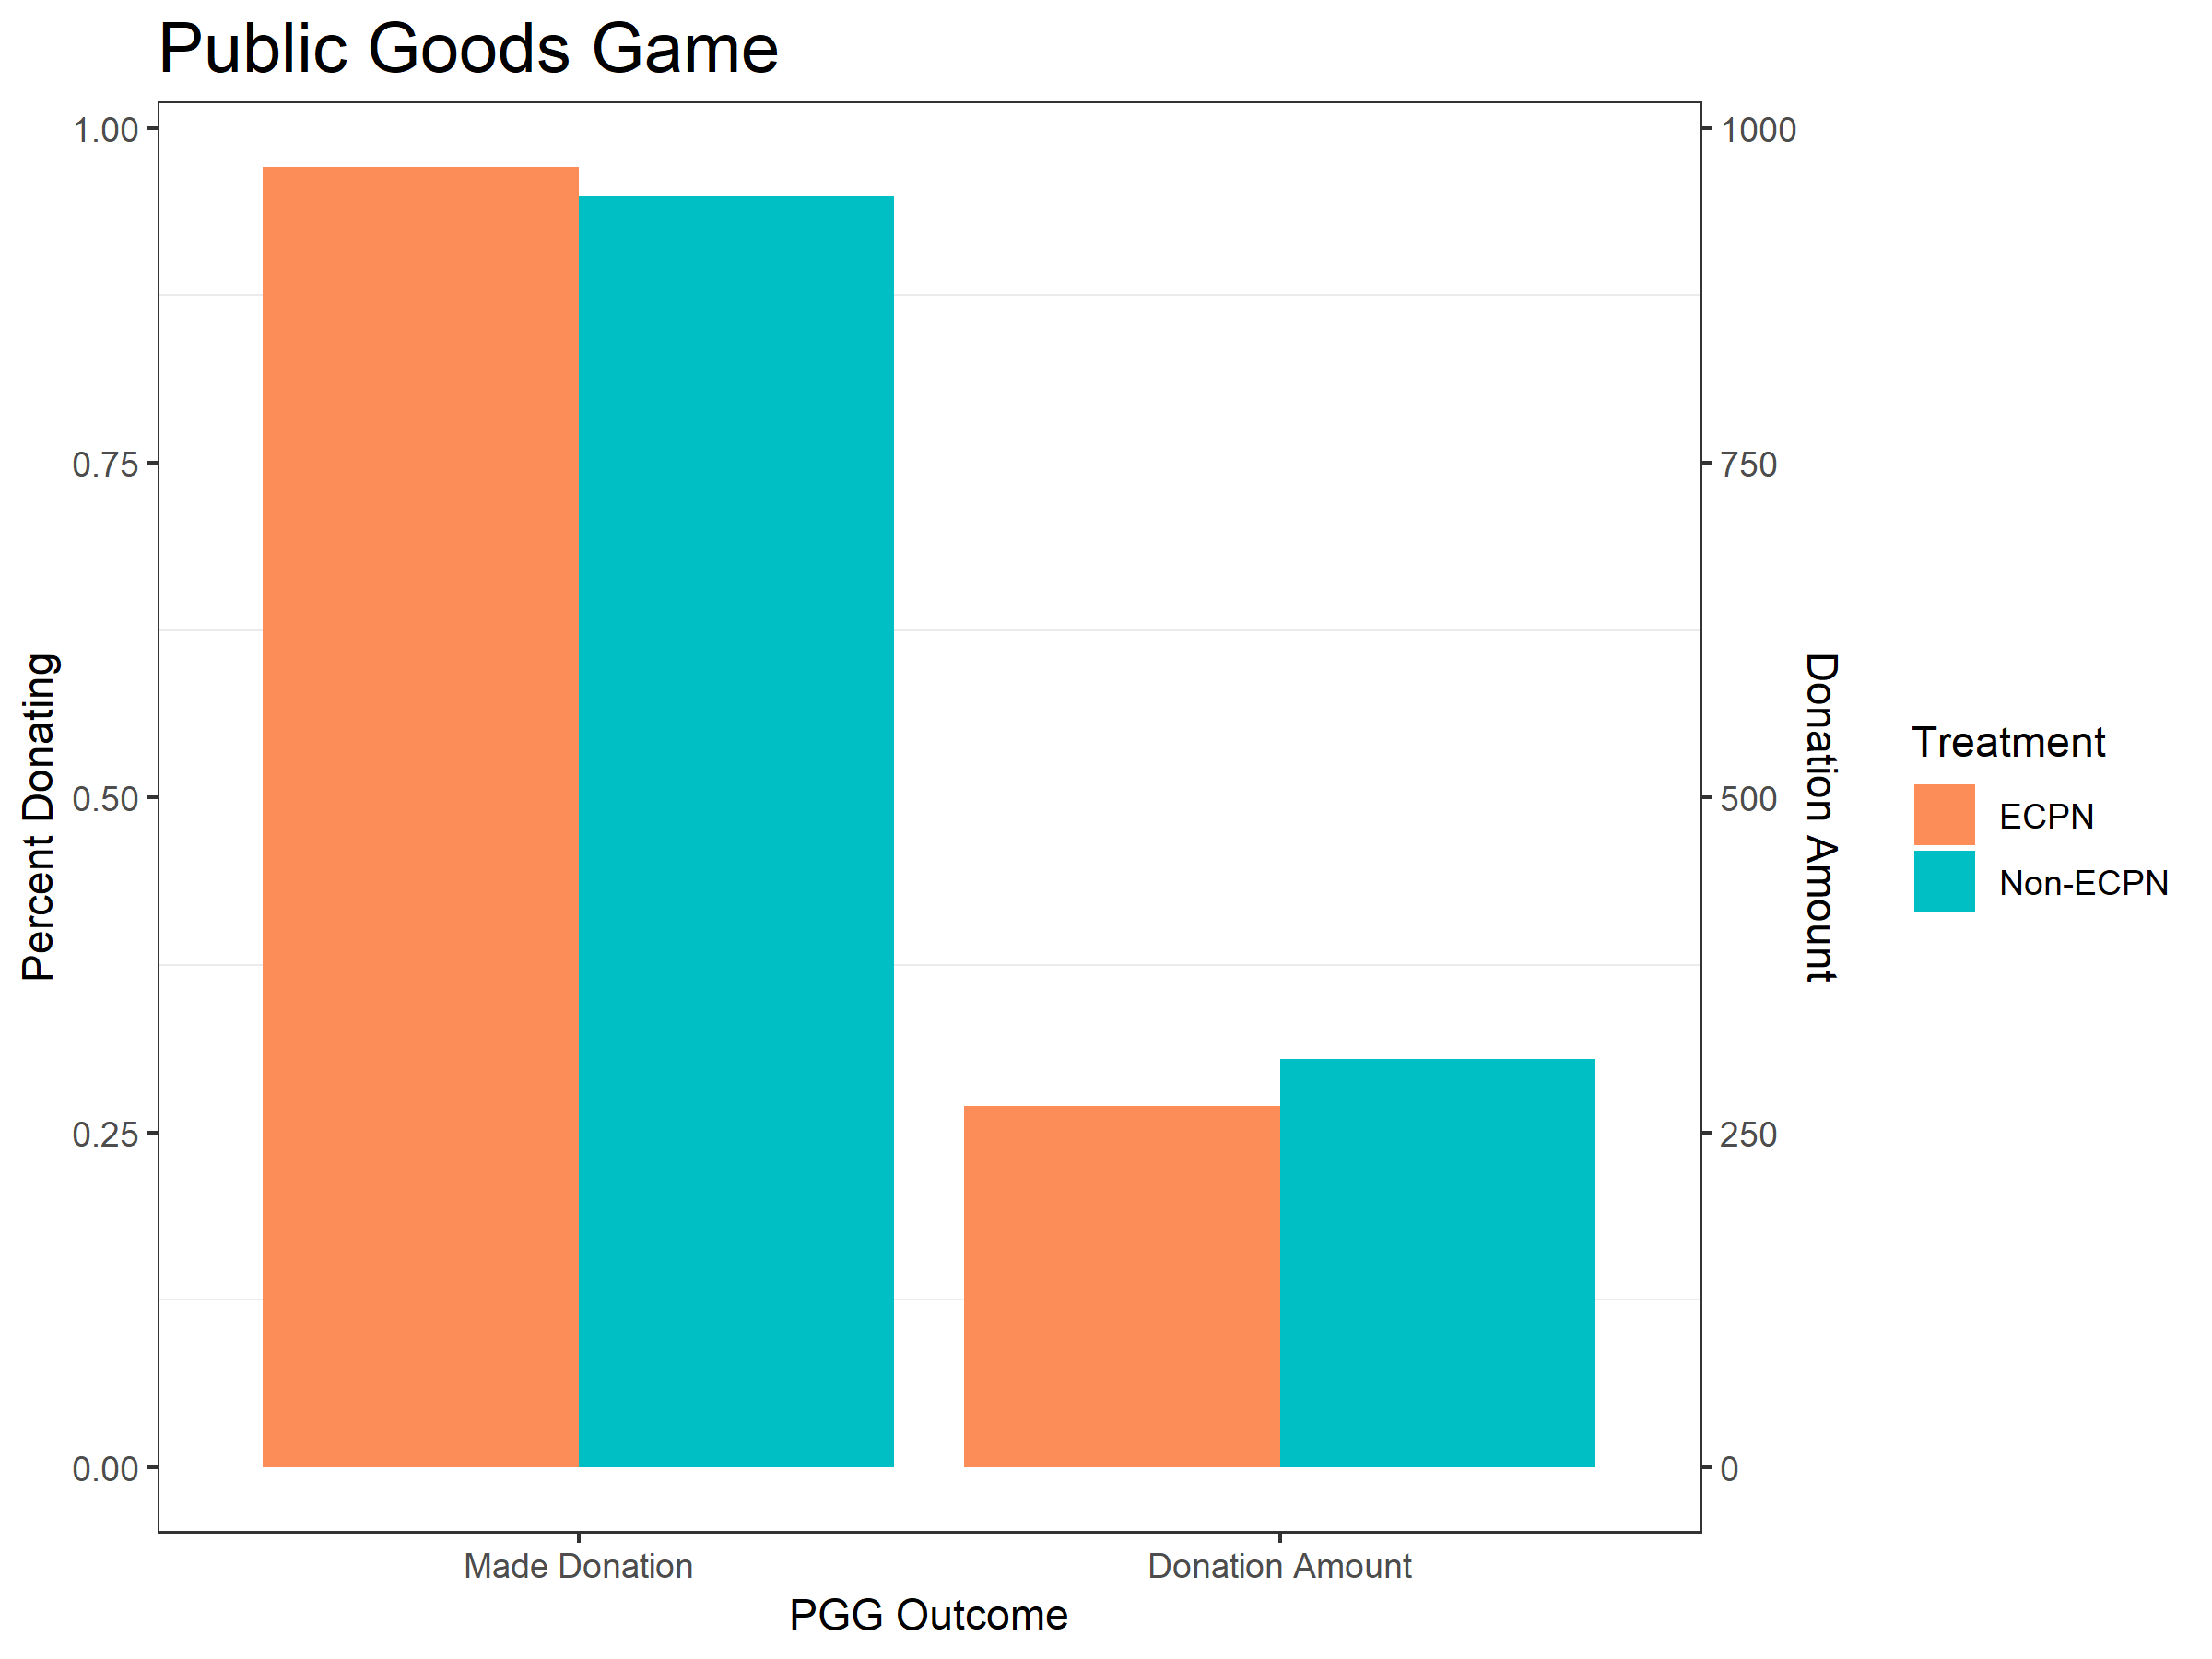
\includegraphics[width=.8\textwidth]{figs/pggComm_plot.png}
\caption{\label{fig:pgg_plot_comm} \textbf{Community Public Goods Game} This figure shows the proportion of each experimental group who donated and their average donation amount. Orange shows the treatment communities; blue shows control communities.}
\end{center}
\end{figure}

\hypertarget{appendix-c-robustness-checks-for-individual-analysis}{%
\subsection{Appendix C: Robustness checks for individual
analysis}\label{appendix-c-robustness-checks-for-individual-analysis}}

These tables shows results with different ways of making indices
(additive vs inverse-covariance weighted), different models for
estimating effects (differencing vs controlling-for), and different ways
of coding count variables (raw vs ranked). Each table is an outcome.
Rows are results for different ways of creating the outcomes. Columns
show the coefficient from OLS regression, true p-value from
randomization inference, and a binary ``base'' indicator showing which
method was used in the paper.

The base method is always inverse-covariance weighted indices; the
estimation method is controlling-for unless the baseline difference
between the participants and control groups is 0.20 standard deviations
or more; the base method of handling count variables is dense rank. Only
contact outcomes use count variables, only survey outcomes have a
baseline and an endline and are measured with indices.

\begin{table}[H]
\begin{center}
\label{tab:attitude_tab_ind}
\caption{\textbf{Individual Attitudes.} Effect of ECPN on attitudes using alternative methods of estimation and index construction. The first column shows coefficients from OLS regression, the second column shows $p$-values from randomization inference, and the third column shows which method was used in the paper.}
\smallskip

\begin{tabular}{l|r|r|r}
\hline
  & coefficient & p-value & base\\
\hline
Non: Controlling-for \& ICW & 0.031 & 0.264 & 0\\
\hline
Part: Controlling-for \& ICW & 0.058 & 0.129 & 0\\
\hline
Non: Controlling-for \& Additive & 0.154 & 0.202 & 0\\
\hline
Part: Controlling-for \& Additive & 0.269 & 0.081 & 0\\
\hline
Non: Differencing \& ICW & 0.054 & 0.130 & 1\\
\hline
Part: Differencing \& ICW & 0.060 & 0.130 & 1\\
\hline
Non: Differencing \& Additive & 0.183 & 0.144 & 0\\
\hline
Part: Differencing \& Additive & 0.296 & 0.049 & 0\\
\hline
\end{tabular}


\end{center}
\end{table}

\begin{table}[H]
\begin{center}
\label{tab:security_tab_ind}
\caption{\textbf{Individual Perceptions of Security} Effect of ECPN on perceptions of security using alternative methods of estimation and index construction. The first column shows coefficients from OLS regression, the second column shows $p$-values from randomization inference, and the third column shows which method was used in the paper.}
\smallskip

\begin{tabular}{l|r|r|r}
\hline
  & coefficient & p-value & base\\
\hline
Non: Controlling-for \& ICW & -0.022 & 0.681 & 0\\
\hline
Part: Controlling-for \& ICW & -0.024 & 0.675 & 0\\
\hline
Non: Controlling-for \& Additive & 0.015 & 0.467 & 0\\
\hline
Part: Controlling-for \& Additive & -0.007 & 0.540 & 0\\
\hline
Non: Differencing \& ICW & 0.045 & 0.178 & 1\\
\hline
Part: Differencing \& ICW & 0.050 & 0.186 & 1\\
\hline
Non: Differencing \& Additive & 0.083 & 0.244 & 0\\
\hline
Part: Differencing \& Additive & 0.146 & 0.123 & 0\\
\hline
\end{tabular}


\end{center}
\end{table}

\begin{table}[H]
\begin{center}
\label{tab:contact_tab_ind}
\caption{\textbf{Individual Contact} Effect of ECPN on contact using alternative methods of estimation, index construction, and measuring count variables. The first column shows coefficients from OLS regression, the second column shows $p$-values from randomization inference, and the third column shows which method was used in the paper.}
\smallskip

\begin{tabular}{l|r|r|r}
\hline
  & coefficient & p-value & base\\
\hline
Non: Controlling-for \& ICW \& Ranks & -0.029 & 0.735 & 0\\
\hline
Part: Controlling-for \& ICW \& Ranks & 0.062 & 0.094 & 0\\
\hline
Non: Controlling-for \& Additive \& Ranks & -0.024 & 0.771 & 0\\
\hline
Part: Controlling-for \& Additive \& Ranks & 0.041 & 0.094 & 0\\
\hline
Non: Differencing \& ICW \& Ranks & 0.002 & 0.492 & 1\\
\hline
Part: Differencing \& ICW \& Ranks & 0.098 & 0.018 & 1\\
\hline
Non: Differencing \& Additive \& Ranks & -0.005 & 0.580 & 0\\
\hline
Part: Differencing \& Additive \& Ranks & 0.063 & 0.017 & 0\\
\hline
Non: Controlling-for \& ICW \& Categories & -0.045 & 0.764 & 0\\
\hline
Part: Controlling-for \& ICW \& Categories & 0.063 & 0.203 & 0\\
\hline
Non: Controlling-for \& ICW \& Raw & -0.023 & 0.737 & 0\\
\hline
Part: Controlling-for \& ICW \& Raw & 0.044 & 0.126 & 0\\
\hline
Non: Differencing \& ICW \& Categories & 0.017 & 0.407 & 0\\
\hline
Part: Differencing \& ICW \& Categories & 0.130 & 0.029 & 0\\
\hline
Non: Differencing \& ICW \& Raw & -0.002 & 0.531 & 0\\
\hline
Part: Differencing \& ICW \& Raw & 0.066 & 0.025 & 0\\
\hline
\end{tabular}


\end{center}
\end{table}

\begin{table}[H]
\begin{center}
\label{tab:pgg_tab_ind}
\caption{\textbf{Individual Publid Goods Game} Effect of ECPN on probability of donating and on donation amount. The first column shows coefficients from OLS regression and the second column shows $p$-values from randomization inference.}
\smallskip

\begin{tabular}{l|r|r}
\hline
  & coefficient & p-value\\
\hline
Non: Donation (binary) & 0.050 & 0.081\\
\hline
Part: Donation (binary) & 0.020 & 0.295\\
\hline
Non: Donation amount & -27.023 & 0.743\\
\hline
Part: Donation amount & -53.740 & 0.875\\
\hline
\end{tabular}


\end{center}
\end{table}

\begin{figure}[H]
\begin{center}
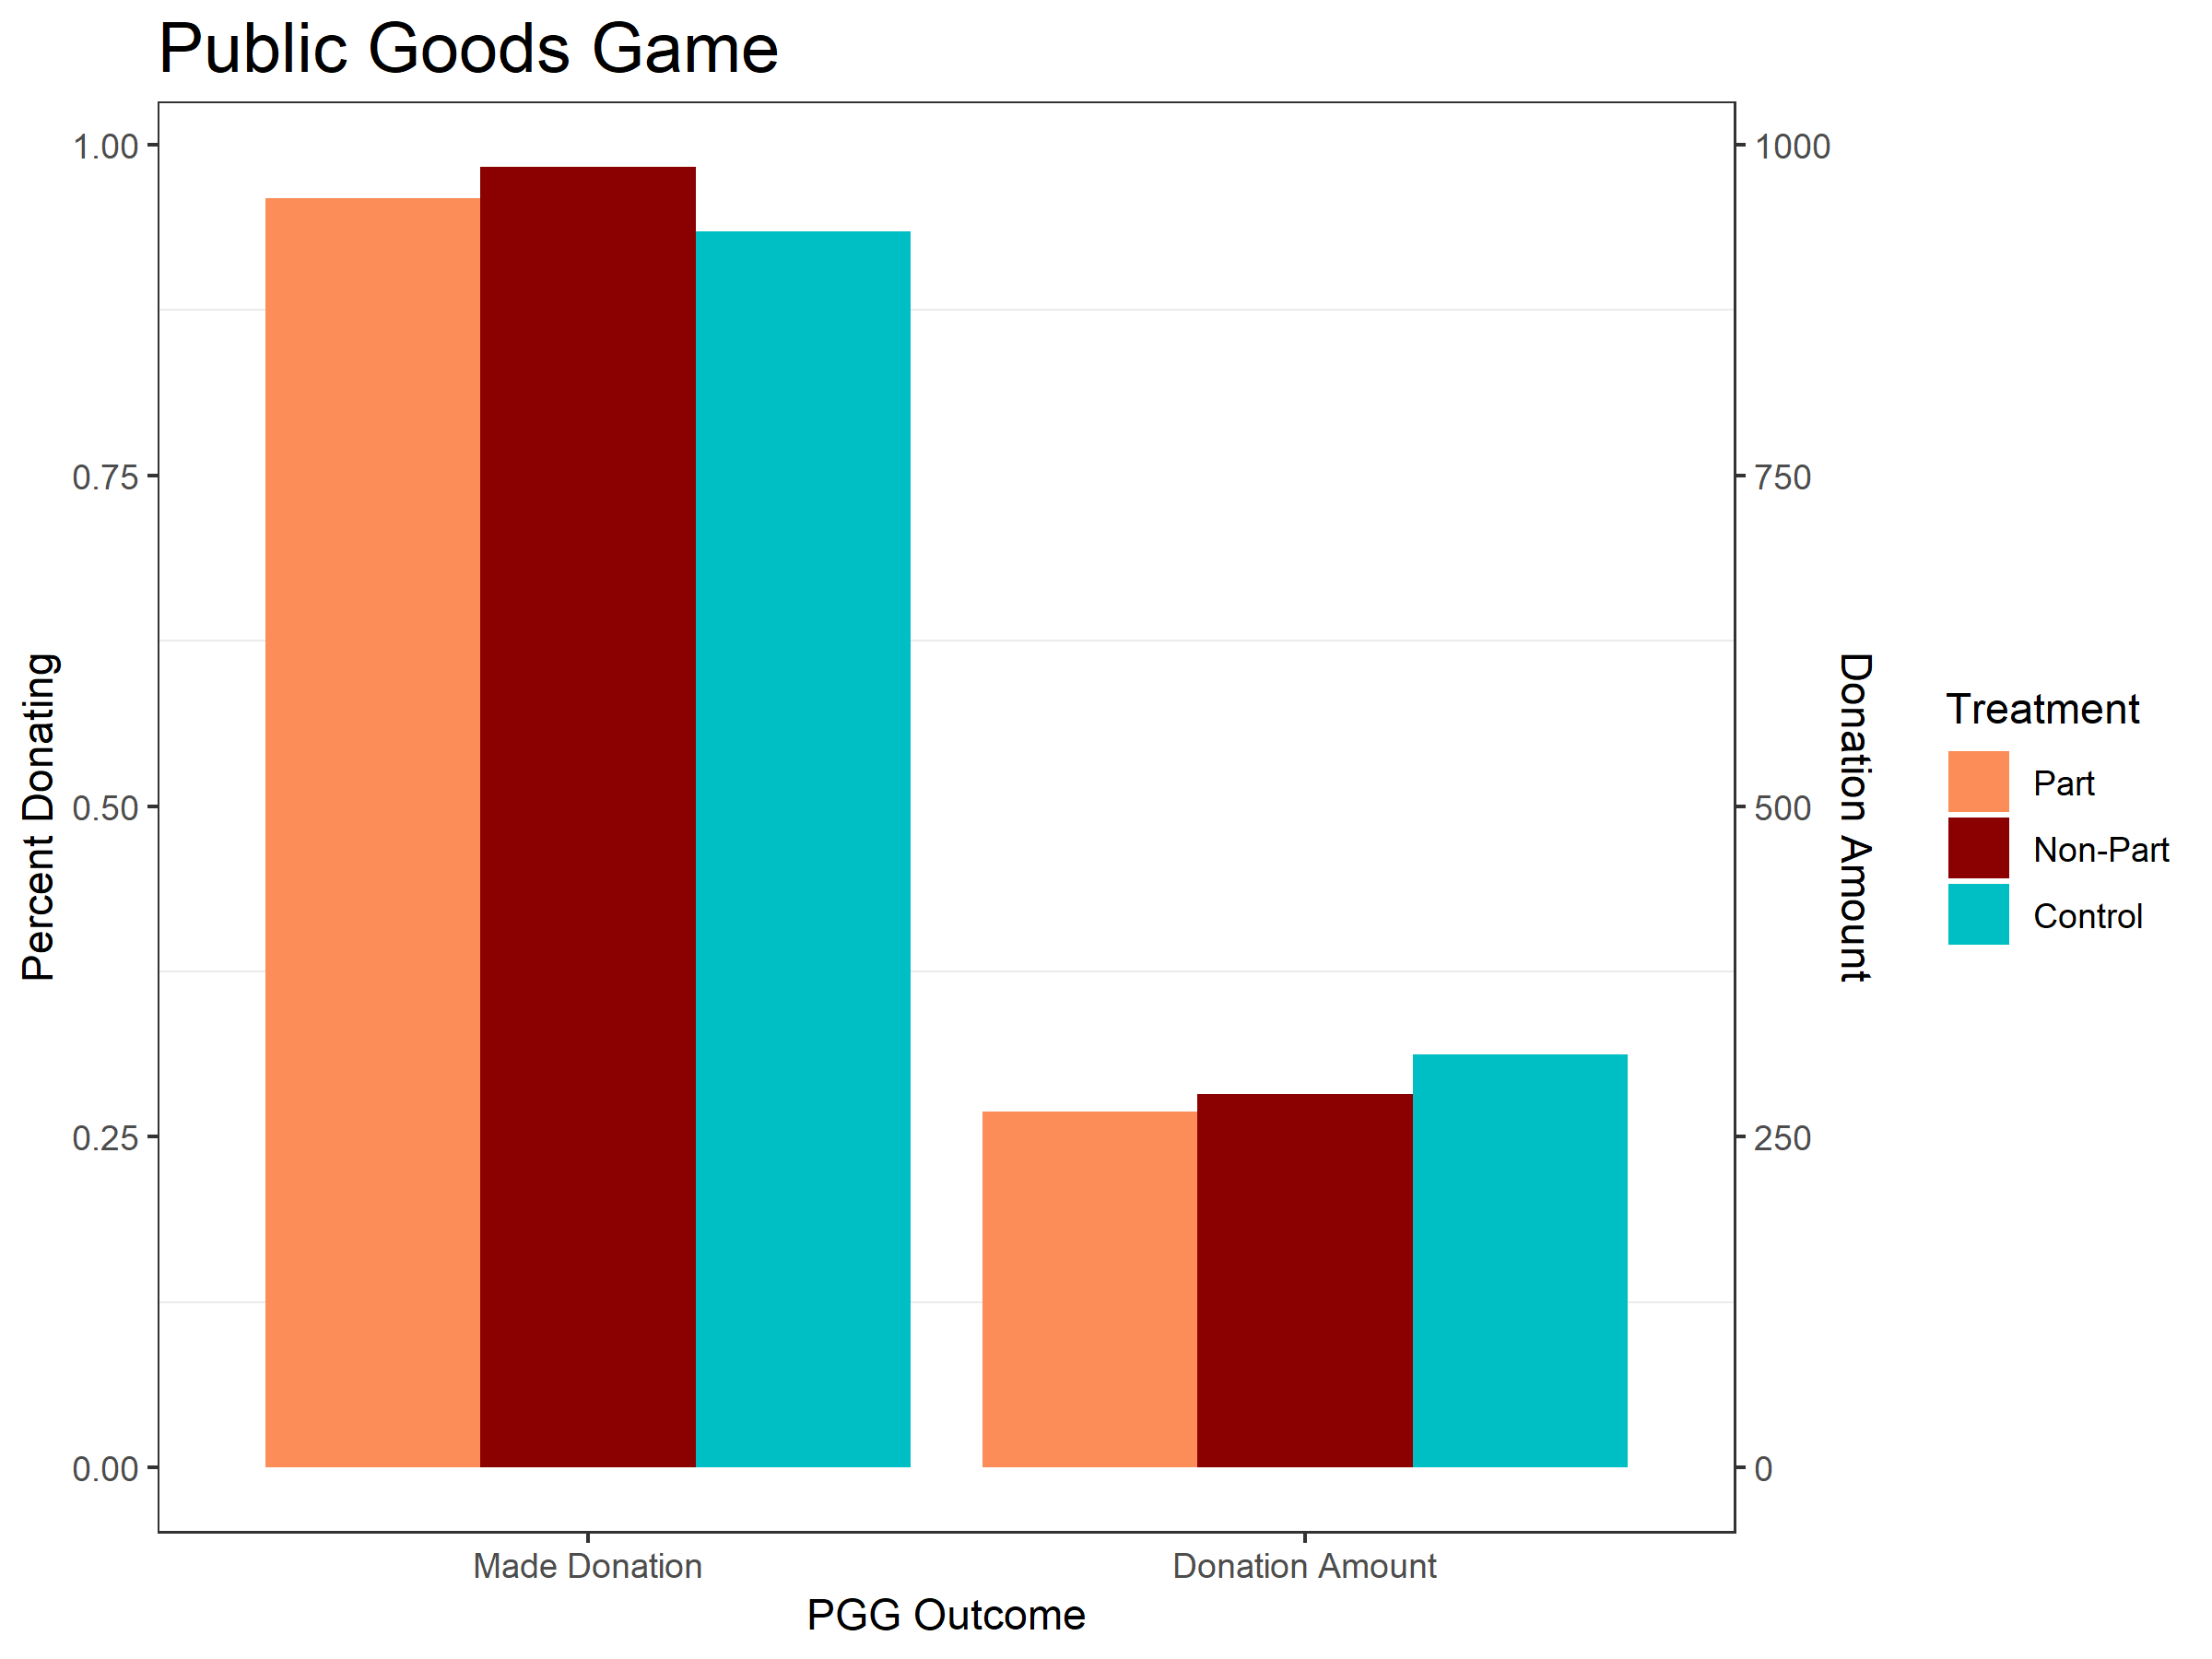
\includegraphics[width=.8\textwidth]{figs/pggPan_plot.png}
\caption{\label{fig:pgg_plot_ind} \textbf{Individual Public Goods Game} This figure shows the proportion of each experimental group who donated and their average donation amount. Orange shows the full participants; red shows the nonparticipants in intervention communities; blue shows people in control communities.}
\end{center}
\end{figure}

\begin{figure}[H]
\begin{center}
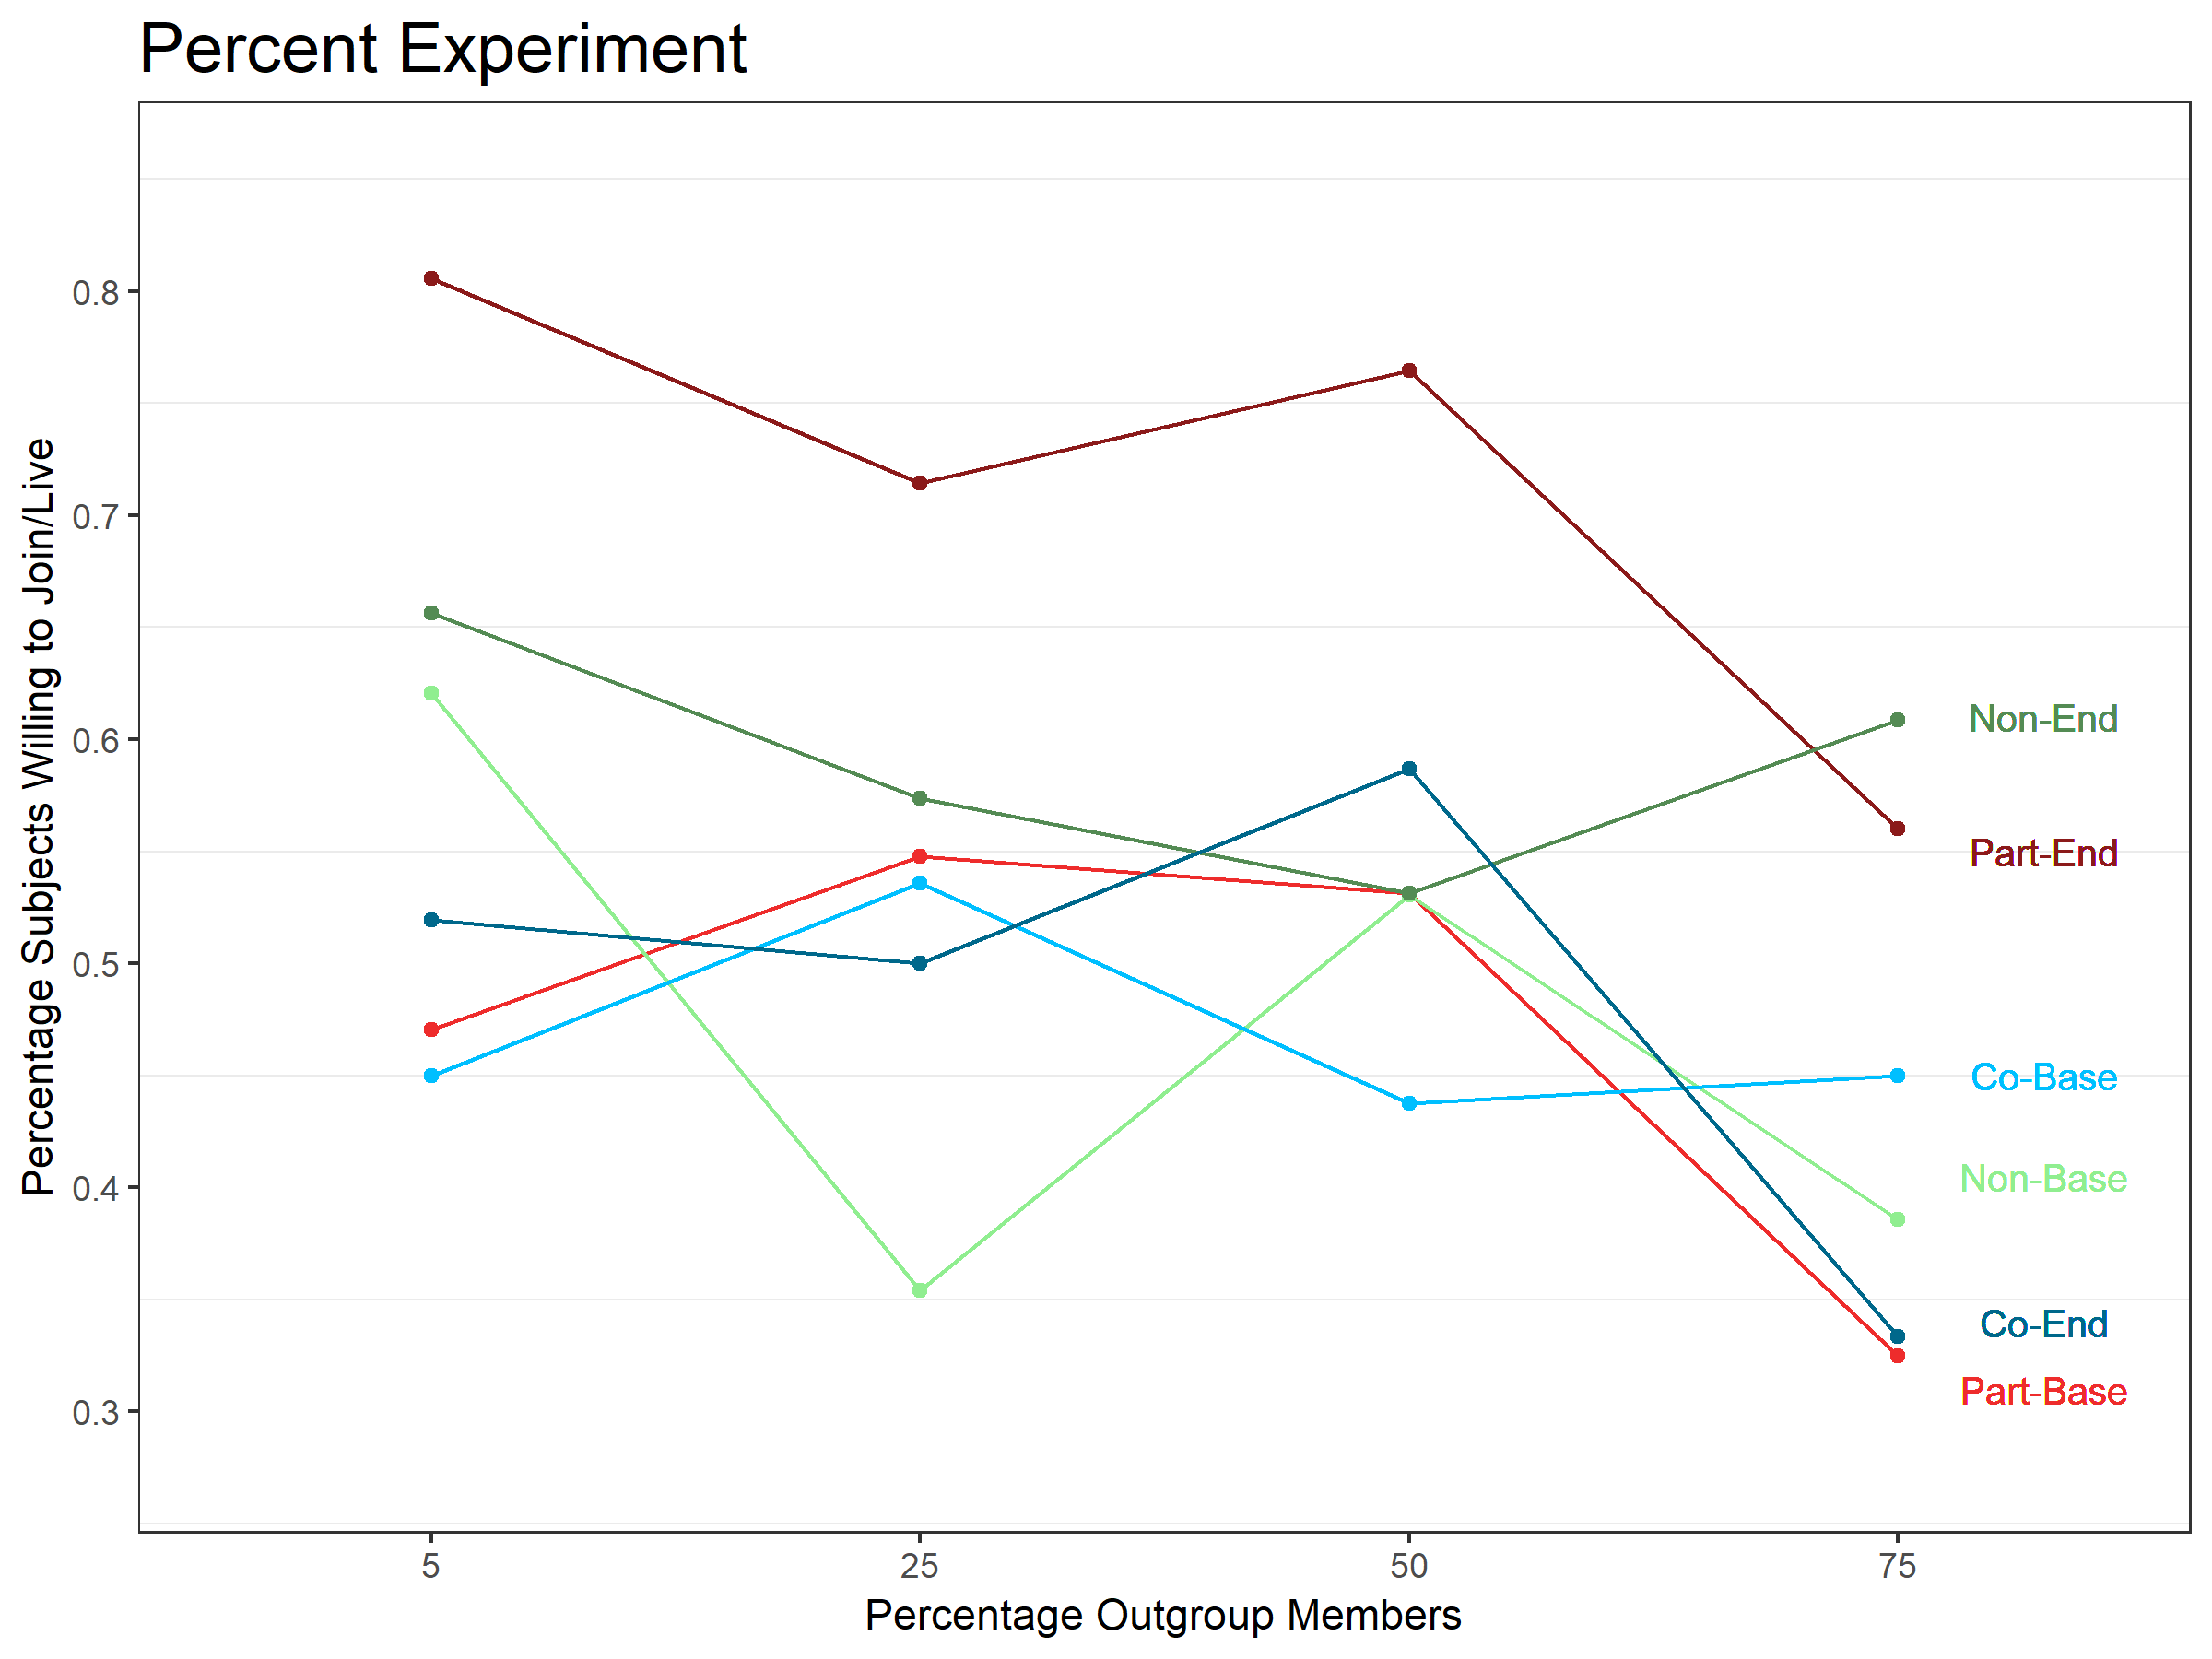
\includegraphics[width=.8\textwidth]{figs/randPan_plot.png}
\caption{\label{fig:percExp_plot_ind} \textbf{Individual Percent Experiment} This figure shows the proportion of each experimental group who would join a group or live in a community with increasing percentages of outgroup members. The outcome is the mean response of those two questions so that a respondent saying yes to both was assigned a 1, a respondent saying yes to one was assigned a 0.5, and a respondent saying no to both was assigned a 0. Red shows the full participants; green shows participants in intervention communities; blue shows control communities.  Light colors are values at baseline; dark colors are values at endline.}
\end{center}
\end{figure}

\hypertarget{appendix-d-balance-tests}{%
\subsection{Appendix D: Balance Tests}\label{appendix-d-balance-tests}}

\begin{table}[H]
\begin{center}
\label{tab:bal_obs_tab1}
\caption{\textbf{Balance: Observational Data All Outcomes}}
\smallskip

\begin{tabular}{l|r|r|r|r|r|r|r}
\hline
  & Control.strat & Treatment.strat & adj.diff.strat & adj.diff.null.sd.strat & std.diff.strat & z.strat & p.strat\\
\hline
Pastoralists\_index\_rank\_events & 35.415 & 25.141 & -10.275 & 12.377 & -0.585 & -0.830 & 0.406\\
\hline
Farmers\_index\_rank\_events & 32.978 & 36.182 & 3.204 & 7.104 & 0.303 & 0.451 & 0.652\\
\hline
Pastoralists\_index\_rank\_markets & 25.458 & 14.151 & -11.308 & 6.576 & -1.375 & -1.720 & 0.086\\
\hline
Farmers\_index\_rank\_markets & 24.417 & 25.250 & 0.834 & 5.699 & 0.101 & 0.146 & 0.884\\
\hline
\end{tabular}


\end{center}
\end{table}

\begin{table}[H]
\begin{center}
\label{tab:bal_obs_tab2}
\caption{\textbf{Balance: Observational Data Omnibus P-value}}
\smallskip

\begin{tabular}{l|r|r|r}
\hline
  & chisquare & df & p.value\\
\hline
strat & 6.494 & 4 & 0.165\\
\hline
\end{tabular}


\end{center}
\end{table}

\begin{table}[H]
\begin{center}
\label{tab:bal_svy_tab1}
\caption{\textbf{Balance: Survey Data All Outcomes}}
\smallskip

\begin{tabular}{l|r|r|r|r|r|r|r}
\hline
  & Control.strat & Treatment.strat & adj.diff.strat & adj.diff.null.sd.strat & std.diff.strat & z.strat & p.strat\\
\hline
Baseline\_Attitudes & 0.542 & 0.566 & 0.023 & 0.065 & 0.098 & 0.357 & 0.721\\
\hline
Baseline\_Perceptions\_of\_Security & -0.459 & -0.537 & -0.079 & 0.071 & -0.246 & -1.113 & 0.266\\
\hline
Baseline\_Contact & 0.496 & 0.336 & -0.159 & 0.104 & -0.585 & -1.528 & 0.127\\
\hline
Baseline\_Percent\_Experiment & 0.443 & 0.474 & 0.031 & 0.056 & 0.206 & 0.543 & 0.587\\
\hline
Baseline\_Endorsement\_Experiment & -0.212 & -0.250 & -0.038 & 0.169 & -0.067 & -0.225 & 0.822\\
\hline
\end{tabular}


\end{center}
\end{table}

\begin{table}[H]
\begin{center}
\label{tab:bal_svy_tab2}
\caption{\textbf{Balance: Survey Data Omnibus P-value}}
\smallskip

\begin{tabular}{l|r|r|r}
\hline
  & chisquare & df & p.value\\
\hline
strat & 6.302 & 5 & 0.278\\
\hline
\end{tabular}


\end{center}
\end{table}

\hypertarget{appendix-e-placebo-tests}{%
\subsection{Appendix E: Placebo tests}\label{appendix-e-placebo-tests}}

Several of our outcomes are survey self-reports, and self-reports could
be affected by factors other than the intervntion. For example, our
survey results are suspect if respondents in treatment communities
learned the ``correct'\,' answers better than respondents in control
communities (social desirability bias). If social desirability accounts
for the effect in survey self-reports, we would also expect differences
between treatment and control for other normatively desirable attitudes.

To test social desirability effects, we conduct a placebo analysis using
attitudes about violence as a placebo. Attitudes about violence are a
good candidate for this placebo because intergroup contact should not
affect general attitudes about violence, but respondents may feel social
pressure to answer violence questions in a desirable way. We measure
attitudes about violence with a six question index asking respondents if
it is always, sometimes, rarely, or never justified to use violence in
certain situations, such as retaliating against violence or bringing
criminals to justice.

Respondents in treatment communities might also express more positive
attitudes towards the outgroup if attitudes were becoming more tolerant
in treatment villages in a way that was unrelated to the intervention.
If attitudes towards any outgroup were becoming more tolerant in
treatment communities compared to control communities, we would expect
attitudes towards religious outgroups to improve more in treatment
communities than control communities. The contact intervention should
not affect attitudes towards people from other religions because the
farmers and pastoralists are often the same religion.

Respondents in treatment communities also might have had better access
to information, and that information changed their
attitudes/perceptions. To measure access to information, we use
frequency of radio listening. If the treatment communities increased
their amount of radio listening significantly more than control
communities, it is possible their attitudes/perceptions changed due to
information and not the contact intervention.

Coefficients come from OLS regression equation specified in the paper
(using state-level blocked fixed effects). P-values come from the
randomization inference described in the paper and in Appendix A; they
are one-sided ``greater-than'' p-values. The base method used in the
paper always constructs indices using inverse-covariance weighting; it
uses the controlling-for method of difference-in-differences estimation
when an outcome's baseline difference between treatment and control is
less than 0.20 standard deviations; it uses the differencing method when
the baseline difference is 0.20 standard deviations or larger.

\hypertarget{community.}{%
\subsubsection{Community.}\label{community.}}

\begin{table}[H]
\begin{center}
\label{tab:pl_vio_tab}
\caption{\textbf{Community Placebo: Attitudes towards violence index.} Effect of ECPN on placebo outcome using alternative methods of estimation and index construction. The first column shows coefficients from OLS regression, the second column shows $p$-values from randomization inference, and the third column shows which method was used in the paper.}
\smallskip

\begin{tabular}{l|r|r|r}
\hline
  & coefficient & p-value & base\\
\hline
Controlling-for \& ICW & 0.010 & 0.466 & 0\\
\hline
Controlling-for \& Additive & 0.004 & 0.441 & 0\\
\hline
Differencing \& ICW & -0.067 & 0.687 & 1\\
\hline
Differencing \& Additive & -0.027 & 0.679 & 0\\
\hline
\end{tabular}


\end{center}
\end{table}

\begin{table}[H]
\begin{center}
\label{tab:pl_vio_tab1}
\caption{\textbf{Community Placebo: Components of violence index.} Effect of ECPN on components of placebo index (attitudes towards violence) using alternative methods of estimation and index construction. The first column shows coefficients from OLS regression, the second column shows $p$-values from randomization inference, and the third column shows which method was used in the paper.}
\smallskip

\begin{tabular}{l|r|r|r}
\hline
  & coefficient & p-value & base\\
\hline
Bring criminals to justice: Controlling-for & 0.034 & 0.252 & 0\\
\hline
Bring criminals to justice: Differencing & -0.092 & 0.792 & 1\\
\hline
Defend ones group: Controlling-for & -0.026 & 0.659 & 1\\
\hline
Defend ones group: Differencing & -0.026 & 0.663 & 0\\
\hline
Defend ones religion: Controlling-for & -0.031 & 0.662 & 1\\
\hline
Defend ones religion: Differencing & -0.031 & 0.671 & 0\\
\hline
Force the government to change their policies: Controlling-for & 0.004 & 0.436 & 1\\
\hline
Force the government to change their policies: Differencing & -0.012 & 0.640 & 0\\
\hline
Maintain culture and traditions: Controlling-for & -0.004 & 0.558 & 1\\
\hline
Maintain culture and traditions: Differencing & -0.011 & 0.585 & 0\\
\hline
Retaliate against violence: Controlling-for & -0.007 & 0.658 & 1\\
\hline
Retaliate against violence: Differencing & 0.011 & 0.387 & 0\\
\hline
\end{tabular}


\end{center}
\end{table}

\begin{table}[H]
\begin{center}
\label{tab:pl_out_tab}
\caption{\textbf{Community Placebo: Trust towards religious outgroups.} Effect of ECPN on placebo outcome using alternative methods of estimation and index construction. The first column shows coefficients from OLS regression, the second column shows $p$-values from randomization inference, and the third column shows which method was used in the paper.}
\smallskip

\begin{tabular}{l|r|r|r}
\hline
  & coefficient & p-value & base\\
\hline
Controlling-for & 0.017 & 0.349 & 1\\
\hline
Differencing & -0.002 & 0.519 & 0\\
\hline
\end{tabular}


\end{center}
\end{table}

\begin{table}[H]
\begin{center}
\label{tab:pl_rad_tab}
\caption{\textbf{Community Placebo: Radio listening frequency.} Effect of ECPN on placebo outcome using alternative methods of estimation and index construction. The first column shows coefficients from OLS regression, the second column shows $p$-values from randomization inference, and the third column shows which method was used in the paper.}
\smallskip

\begin{tabular}{l|r|r|r}
\hline
  & coefficient & p-value & base\\
\hline
Controlling-for & 0.021 & 0.430 & 1\\
\hline
Differencing & 0.021 & 0.441 & 0\\
\hline
\end{tabular}


\end{center}
\end{table}

\hypertarget{individual}{%
\subsubsection{Individual}\label{individual}}

\begin{table}[H]
\begin{center}
\label{tab:pl_vio_ind}
\caption{\textbf{Individual Placebo: Attitudes towards violence index.} Effect of ECPN on placebo outcome using alternative methods of estimation and index construction. The first column shows coefficients from OLS regression, the second column shows $p$-values from randomization inference, and the third column shows which method was used in the paper.}
\smallskip

\begin{tabular}{l|r|r|r}
\hline
  & coefficient & p-value & base\\
\hline
Non: Controlling-for \& ICW & -0.057 & 0.801 & 0\\
\hline
Part: Controlling-for \& ICW & 0.013 & 0.413 & 0\\
\hline
Non: Controlling-for \& Additive & -0.163 & 0.770 & 0\\
\hline
Part: Controlling-for \& Additive & 0.022 & 0.441 & 0\\
\hline
Non: Differencing \& ICW & -0.033 & 0.642 & 1\\
\hline
Part: Differencing \& ICW & -0.016 & 0.549 & 1\\
\hline
Non: Differencing \& Additive & -0.058 & 0.580 & 0\\
\hline
Part: Differencing \& Additive & -0.023 & 0.508 & 0\\
\hline
\end{tabular}


\end{center}
\end{table}

\begin{table}[H]
\begin{center}
\label{tab:pl_vio_ind1}
\caption{\textbf{Individual Placebo: Components of violence index.} Effect of ECPN on components of placebo index (attitudes towards violence) using alternative methods of estimation and index construction. The first column shows coefficients from OLS regression, the second column shows $p$-values from randomization inference, and the third column shows which method was used in the paper.}
\smallskip

\begin{tabular}{l|r|r|r}
\hline
  & coefficient & p-value & base\\
\hline
Non: Bring criminals to justice: Controlling-for & -0.154 & 0.680 & 0\\
\hline
Part: Bring criminals to justice: Controlling-for & -0.031 & 0.535 & 0\\
\hline
Non: Bring criminals to justice: Differencing & -0.292 & 0.813 & 1\\
\hline
Part: Bring criminals to justice: Differencing & -0.494 & 0.933 & 1\\
\hline
Non: Defend ones group: Controlling-for & -0.078 & 0.616 & 1\\
\hline
Part: Defend ones group: Controlling-for & 0.039 & 0.440 & 1\\
\hline
Non: Defend ones group: Differencing & 0.034 & 0.447 & 0\\
\hline
Part: Defend ones group: Differencing & -0.021 & 0.525 & 0\\
\hline
Non: Defend ones religion: Controlling-for & -0.250 & 0.892 & 1\\
\hline
Part: Defend ones religion: Controlling-for & 0.141 & 0.276 & 1\\
\hline
Non: Defend ones religion: Differencing & -0.143 & 0.726 & 0\\
\hline
Part: Defend ones religion: Differencing & 0.067 & 0.378 & 0\\
\hline
Non: Force the government to change their policies: Controlling-for & -0.227 & 0.781 & 1\\
\hline
Part: Force the government to change their policies: Controlling-for & 0.031 & 0.457 & 1\\
\hline
Non: Force the government to change their policies: Differencing & -0.142 & 0.684 & 0\\
\hline
Part: Force the government to change their policies: Differencing & 0.013 & 0.496 & 0\\
\hline
Non: Maintain culture and traditions: Controlling-for & -0.190 & 0.797 & 1\\
\hline
Part: Maintain culture and traditions: Controlling-for & 0.024 & 0.443 & 1\\
\hline
Non: Maintain culture and traditions: Differencing & 0.022 & 0.453 & 0\\
\hline
Part: Maintain culture and traditions: Differencing & 0.161 & 0.261 & 0\\
\hline
Non: Retaliate against violence: Controlling-for & -0.091 & 0.639 & 1\\
\hline
Part: Retaliate against violence: Controlling-for & -0.080 & 0.601 & 1\\
\hline
Non: Retaliate against violence: Differencing & 0.176 & 0.254 & 0\\
\hline
Part: Retaliate against violence: Differencing & 0.156 & 0.286 & 0\\
\hline
\end{tabular}


\end{center}
\end{table}

\begin{table}[H]
\begin{center}
\label{tab:pl_out_ind}
\caption{\textbf{Individual Placebo: Trust towards religious outgroups.} Effect of ECPN on placebo outcome using alternative methods of estimation and index construction. The first column shows coefficients from OLS regression, the second column shows $p$-values from randomization inference, and the third column shows which method was used in the paper.}
\smallskip

\begin{tabular}{l|r|r|r}
\hline
  & coefficient & p-value & base\\
\hline
Non: Controlling-for & 0.178 & 0.208 & 1\\
\hline
Part: Controlling-for & -0.060 & 0.586 & 1\\
\hline
Non: Differencing & 0.140 & 0.283 & 0\\
\hline
Part: Differencing & -0.079 & 0.616 & 0\\
\hline
\end{tabular}


\end{center}
\end{table}

\begin{table}[H]
\begin{center}
\label{tab:pl_rad_ind}
\caption{\textbf{Individual Placebo: Radio listening frequency.} Effect of ECPN on placebo outcome using alternative methods of estimation and index construction. The first column shows coefficients from OLS regression, the second column shows $p$-values from randomization inference, and the third column shows which method was used in the paper.}
\smallskip

\begin{tabular}{l|r|r|r}
\hline
  & coefficient & p-value & base\\
\hline
Non: Controlling-for & 0.178 & 0.208 & 1\\
\hline
Part: Controlling-for & -0.060 & 0.586 & 1\\
\hline
Non: Differencing & 0.140 & 0.283 & 0\\
\hline
Part: Differencing & -0.079 & 0.616 & 0\\
\hline
\end{tabular}


\end{center}
\end{table}

\hypertarget{appendix-f-state-level-differences}{%
\subsection{Appendix F: State-level
differences}\label{appendix-f-state-level-differences}}

Coefficients and p-values estimating state-level heterogeneous effects
were calculated with robust OLS regression using site-level clusters.
The regression interacted the treatment indicator with the state
indicator. This is a low-power analysis. There are no significant
differences in treatment effect by state. Benue was the reference
category so this table shows differences for Nasarawa.

\begin{table}[H]
\begin{center}
\label{tab:state_tab}
\caption{\textbf{State-level differences in community-level analysis.} There are not significant differences between the effect of the contact intervention by state. The first column shows coefficients from OLS regression, the second column shows $p$-values from OLS regression.}
\smallskip

\begin{tabular}{l|r|r}
\hline
  & coefficient & p-value\\
\hline
Attitudes & -0.176 & 0.315\\
\hline
Perceptions of security & 0.133 & 0.383\\
\hline
Contact & -0.104 & 0.469\\
\hline
Percent Experiment & -0.251 & 0.158\\
\hline
Endorsement Experiment & 0.191 & 0.488\\
\hline
PGG donation & -0.093 & 0.257\\
\hline
PGG amount & -84.807 & 0.442\\
\hline
\end{tabular}


\end{center}
\end{table}

\hypertarget{appendix-g-farmer-pastoralist-differences}{%
\subsection{Appendix G: Farmer-pastoralist
differences}\label{appendix-g-farmer-pastoralist-differences}}

Coefficients and p-values estimating farmer/pastoralist heterogeneous
effects were calculated with robust OLS regression using site-level
clusters and fixed effects for state. The regression interacted the
treatment indicator with the state indicator. There are no significant
differences in treatment effect by farmer/pastoralist. Farmers were the
reference category so this table shows differences for pastoralists.

\begin{table}[H]
\begin{center}
\label{tab:farm_tab}
\caption{\textbf{Farmer-pastoralist differences in community-level analysis.} There are not significant differences between the effect of the contact intervention by farmer/pastoralist. The first column shows coefficients from OLS regression, the second column shows $p$-values from OLS regression.}
\smallskip

\begin{tabular}{l|r|r}
\hline
  & coefficient & p-value\\
\hline
Attitudes & -0.090 & 0.278\\
\hline
Perceptions of security & 0.021 & 0.905\\
\hline
Contact & 0.031 & 0.911\\
\hline
Percent Experiment & -0.014 & 0.913\\
\hline
Endorsement Experiment & -0.194 & 0.626\\
\hline
PGG donation & -0.064 & 0.386\\
\hline
PGG amount & 23.284 & 0.784\\
\hline
\end{tabular}


\end{center}
\end{table}

\begin{center}\rule{0.5\linewidth}{0.5pt}\end{center}

\hypertarget{appendix-z-survey-questions}{%
\subsection{Appendix Z: Survey
Questions}\label{appendix-z-survey-questions}}

\textbf{Attitudes}

\begin{itemize}
\tightlist
\item
  With regards to someone from {[}X GROUP{]}, would you feel
  comfortable:

  \begin{itemize}
  \tightlist
  \item
    if they worked in your field?
  \item
    paying them to watch your animals?
  \item
    trading goods with them?
  \item
    sharing a meal with them?
  \item
    with a close relative marrying a person from {[}X GROUP{]}?
  \end{itemize}
\item
  From 1-5, how much do you trust people from {[}X GROUP{]} in your
  area?
\item
  Now I'm going to ask you questions about your community here in
  Benue/Nassarawa, including {[}X GROUP{]}. Please tell me how strongly
  you agree/disagree with each of the following statements: People in
  this area can be trusted.
\end{itemize}

\textbf{Contact}

\begin{itemize}
\tightlist
\item
  Now I'm going to ask you questions about your contact with {[}X
  GROUP{]} in your area.

  \begin{itemize}
  \tightlist
  \item
    Think of the market you go to most frequently. During the past
    month, have members of X GROUP gone to that market too? In the past
    month, how many times did you interact with X group in the market?
  \end{itemize}
\item
  In the past month, have you:

  \begin{itemize}
  \tightlist
  \item
    Joined a member of X group for a social event outside the home? How
    often?
  \item
    Hosted a member of X group for a ceremony in your home? How often?
  \item
    Gone to the home of a member of X group for a ceremony? How often?
  \item
    Have you interacted with members of X group in any other way in the
    past month?
  \end{itemize}
\end{itemize}

\textbf{Insecurity}

\begin{itemize}
\tightlist
\item
  In the last year were there any areas that you avoided going to or
  through because of insecurity during the night?
\item
  In the last year were there any areas that you avoided going to or
  through because of insecurity, during the day?
\item
  In the last year, did insecurity ever prevent you from:

  \begin{itemize}
  \tightlist
  \item
    Working when you wanted to work? About how many days were you unable
    to work?
  \item
    Going to the market?
  \item
    Getting water for the household?
  \item
    Going to your field/farm?
  \item
    Moving your animals to grazing areas?
  \item
    Moving your animals to water?
  \item
    Earning money or going to work?
  \item
    Going to school?
  \end{itemize}
\end{itemize}

\textbf{Endorsement Experiment}

\begin{itemize}
\tightlist
\item
  Imagine that there is a proposal by {[}\textbf{the Farmer's
  Cooperative Society}/\textbf{MACBAN}{]} for action to enhance access
  to clean water in rural areas. Though expensive, the proposal aims to
  bring fresh, clean water to hundreds of areas without access to it,
  including this one. If this were proposed, how would you feel about
  it?
\end{itemize}

\textbf{Percent Experiemnt}

\begin{itemize}
\tightlist
\item
  Think about groups that you might join in your leisure time. Would you
  join a group that had \textbf{5/25/50/75}\% X Group members?
\item
  Think about the community you live in. Would you live in a community
  that had \textbf{5/25/50/75}\% X Group members?
\end{itemize}

\textbf{Violence Placebo}

\begin{itemize}
\tightlist
\item
  Now I am going to ask you some questions about the use of violence. Is
  it always, sometimes, rarely, or never justified to use violence to do
  each of the following:

  \begin{itemize}
  \tightlist
  \item
    Retaliate against violence
  \item
    Defend one's group
  \item
    Maintain culture and traditions
  \item
    Defend one's religion
  \item
    Bring criminals to justice
  \item
    Force the government to change their policies
  \end{itemize}
\end{itemize}

\textbf{Public Goods Game}

``Thank you very much for participating in our survey. Before I go,
there is one last thing. As you may have heard, we have development
funds to use in this community. We have randomly selected you as one of
the 50 people to receive these funds. These funds are not for a Mercy
Corps project, but rather for you to keep personally or to donate to a
community fund.

We have 1,000 Naira to give to you. It is yours, and you can use it
either way--for yourself or for a community good.

Your community and {[}joint farmer/pastoralist community{]} have created
a project committee to whom you can donate this money so that it may be
used to help both communities. The project committee has 4 people from
each community. We have found a donor that will match the funds that you
all contribute to the project committee, so that if you donate 100 Naira
the project committee receives 300 Naira, and if you donate all 1,000
Naira the project committee receives 3,000 Naira. You are welcome to
donate none, some, or all of the money to the project committee.

These are your individual donation envelopes. All the donations will be
private -- only you will know how much money you donated. It essential
that you keep how much you give private -- please do not tell anyone. I
have with me a donation envelope to collect donations. Please go into
your home, put however much of the 1,000 Naira you wish to donate to the
project committee in the envelope, take whatever amount you want to keep
for yourself, and come back to place your envelope in the donation
envelope. Remember, you are welcome to donate none, some, or all of the
money to the project committee. After that we are finished and you may
continue your day. We will come back and publicly announce how much
money your community's project committee will receive.''

\end{document}
